% Chapter 3

\chapter{State-of-the-art Analysis} % Main chapter title
\label{Chapter3} % For referencing the chapter elsewhere, use \ref{Chapter3} 

\lhead{Chapter 3. \emph{State-of-the-art Analysis}} % This is for the header on each page - perhaps a shortened title

%----------------------------------------------------------------------------------------
% In this section, we discuss the core requirements and other factors that are required to be solved to provide a viable solution. There are plenty of alternatives available under each topic. Thus, we consider solutions that are mostly relevant, widely available and used in the related domain, industry as well as findings from latest related research works. This analysis enables us to choose the best data treatment technique and programming model that are well suited and to select the core design aspects that need to be considered. To make selections with adequate foundation, we first discuss the requirements and then compare each alternatives with respect to the requirements. 
% \section{Requirements }
% \label{sec:fundamentals}
% Essential requirements that need to be met by the system are defined in Section \ref{sec:problem} and additional aspects that needs to be solved by new scalable ETL tools are mentioned in Section \ref{sec:requirements}. To summarize, the system should be execute data preparation on large data (R1), scalable i.e. able to distribute the work according to the load  (R2), real-time responsive in interactive context (R3), efficient on iterative execution (R4). Further, Separation between logical and physical implementation of data cleaning operations becomes an optimization requirement (R5), providing flexibility (R6) behaves as a functional improvement requirement and solution as a service (R7) to provide a general integral solution.  The following important topics need to be carefully analyzed with respect to problem space to create a fit-for-purpose solution. 

% \subsection{Data ingestion technique}
% On small intervals, the incoming stream is collected to a chunk of data and delivered to be processed as a small batch of input \cite{beyondbatchprocessing}. Choice of appropriate data ingestion technique is essential to receive precise output. Given that, on today's date, the messy data we target to process in open data context are usually text-files or spreadsheets. These data are already available and need to be processed to create RDF data. Batch processing is generally used as store-first, process-second model of large and of identical types. In contrast, streams are not considered to be available before it is processed and they can be out-of-order, out-of-streams \cite{beyondbatchprocessing} \cite{Sims-387}. Stream processing is mainly aimed to do continuous processing on similar data streams in real-time \cite{8reqofrealtime} 
% \begin{center}
% 	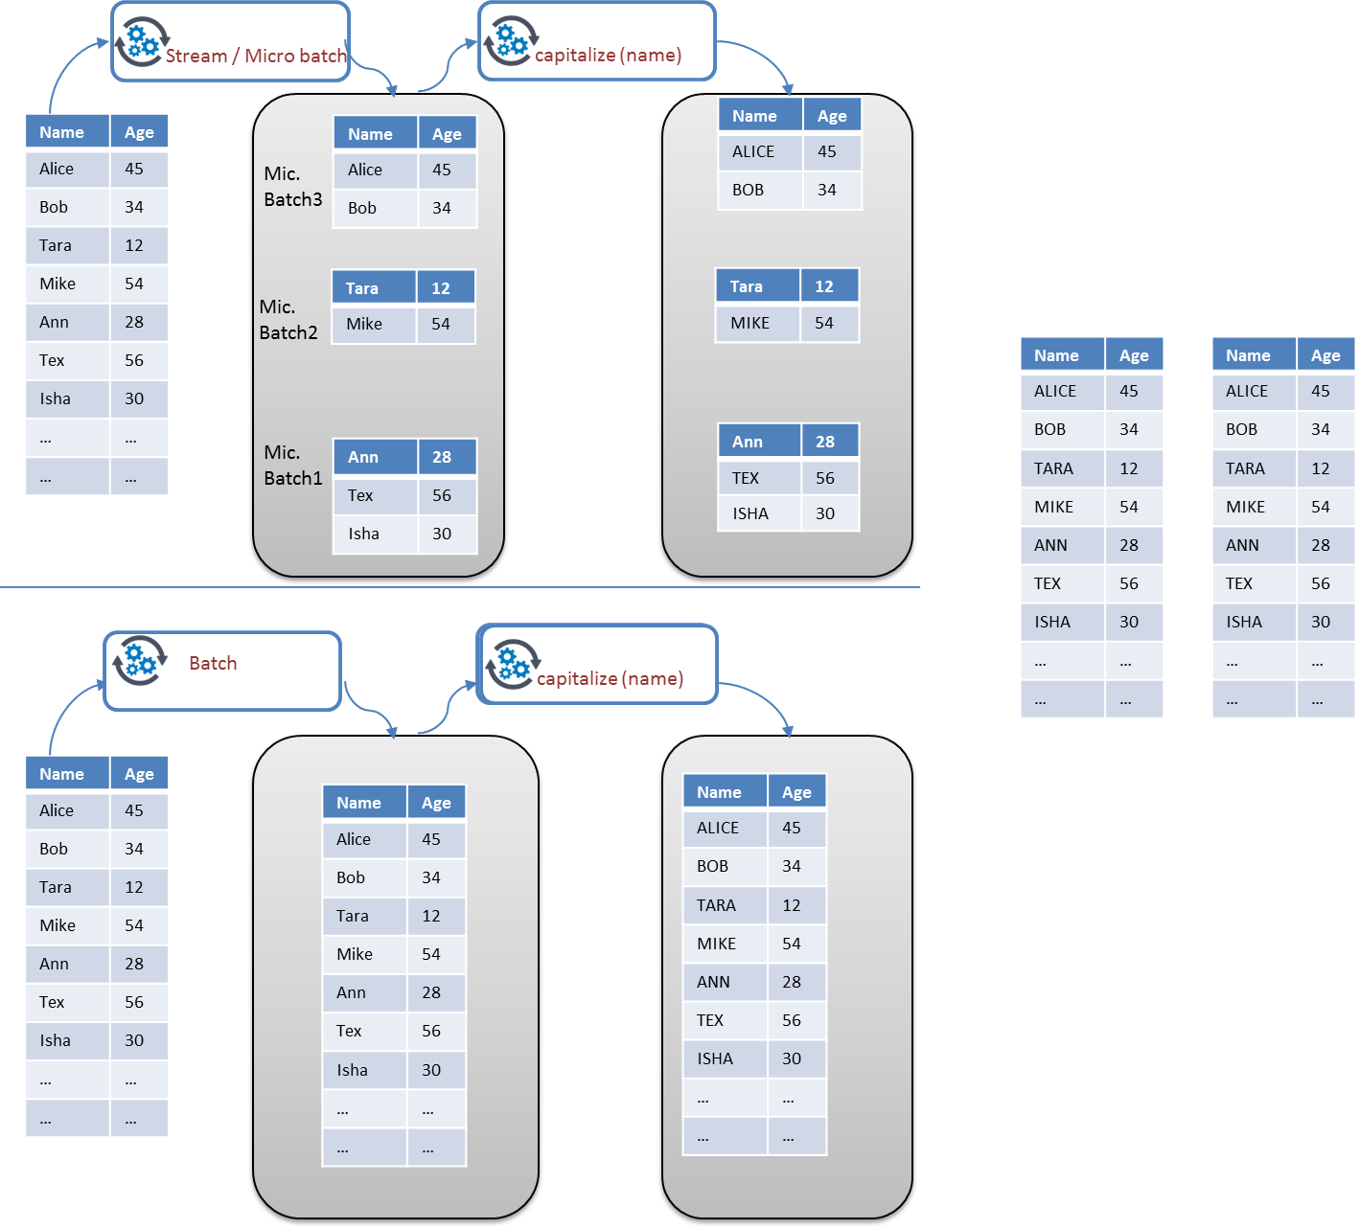
\includegraphics[width=38em]{./Figures/batch-cleaning-right}
% 	\begin{figure}[htbp]
%     \caption{Data cleaning in different data treatment techniques performed as expected}
%     \label{fig:streamcorrect}
% 	\end{figure}
% \end{center}
%  Since we need to process large files, the right choice of data ingestion is important. Streaming or Micro batching data can be a solution to overcome the problem of processing large files. However, since we need to perform ETL operations on table like data, it will not result in expected output in all instances. Figure \ref{fig:streamcorrect} shows that streaming or micro batching can provide expected solution when simple data cleaning operations performed independent from other row values such as capitalize, lower case and upper case etc. 
%  \begin{center}
% 	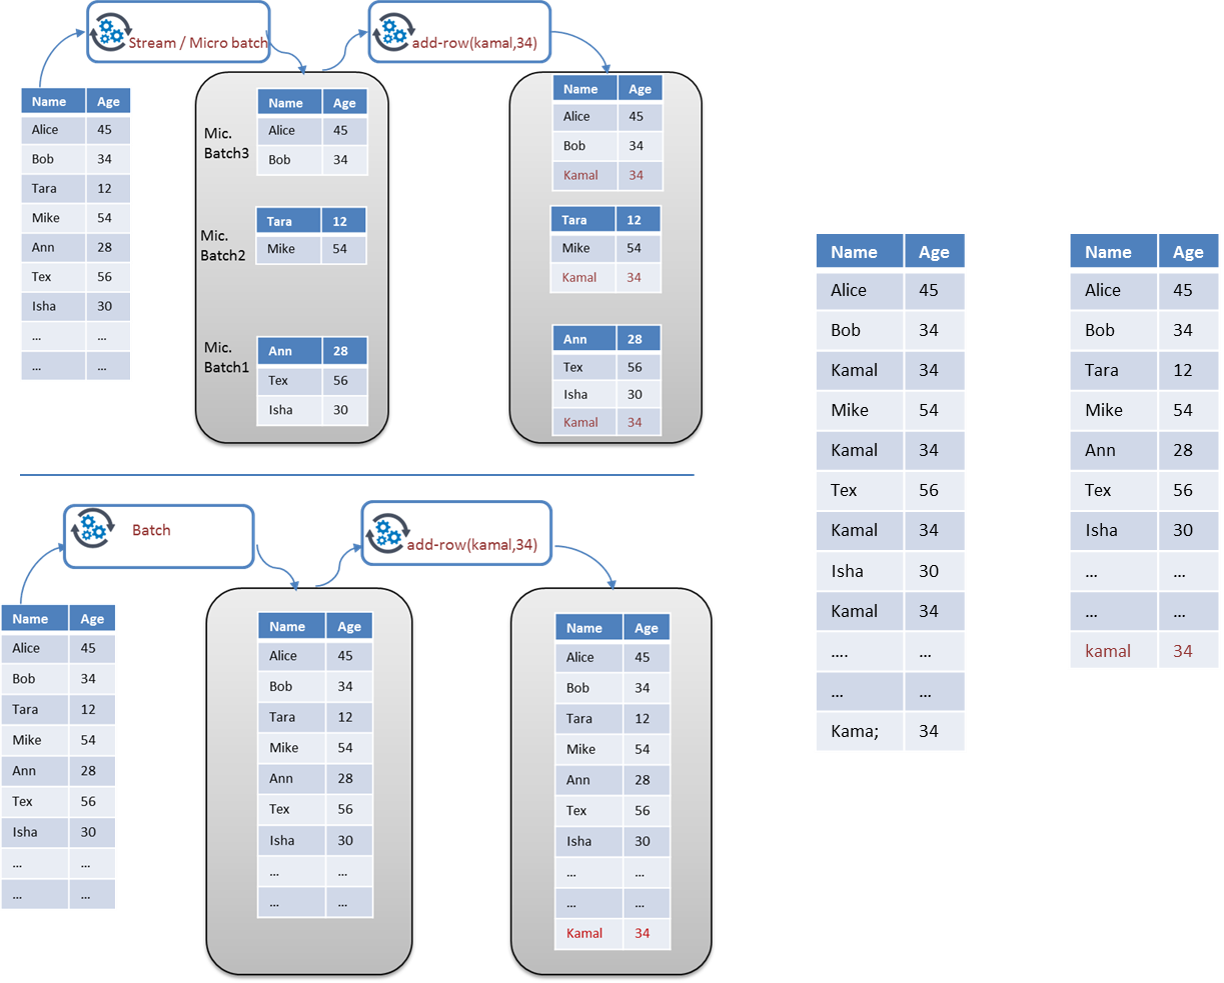
\includegraphics[width=38em]{./Figures/batch-cleaning-wrong}
% 	\begin{figure}[htbp]
%     \caption{Data cleaning on a faulty data treatment results in unexpected result}
%     \label{fig:stream-wrong}
% 	\end{figure}
% \end{center}
%  However, it will result in wrong output when collective operations or row dependent operations like add-row is performed on data as shown in Figure \ref{fig:stream-wrong}. Figure \ref{fig:stream-wrong} illustrates an add-row operation performed on a simple tabular data. When the data is ingested as streams, which are independent from each other, the transformation pipelines are performed on all streams which result in redundant addition of rows, whereas in batch ingestion the data is treated as a single batch and operation is performed safely. Performing complex schema-based data cleaning will be cumbersome and error-prone in stream or micro batch processing. Seeing that, we conclude that ingesting those messy files as batch is the most suitable and precise method for data cleaning. This adds efficient batch-processing (R5) to our requirements. This implicitly requires our solution to process large file as a batch input and respond in real-time. In contrast, batch processing is typically performed as batch jobs which are independent from user \cite{beyondbatchprocessing} and take longer duration (from few minutes to hour) to complete. Despite, we attempt to solve this in near-real-time (i.e within few seconds to few minutes) which can still afford to have active user interaction and perform batch processing. 
% \section{Summary}
% After analyzing important requirements and solution fundamentals, we have noted that batch-processing is the correct ingesting method to do data cleaning on offline messy data. Secondly, in-memory computing and distributed data parallelizatoin from Apache Spark can be exploited to perform interactive, iterative data cleaning. 